\documentclass[a4paper,12pt]{article}
\usepackage{fullpage}
\usepackage{graphicx}
\usepackage{caption}
\usepackage{float}
\usepackage{hyperref}

\hypersetup{
    colorlinks,
    citecolor=blue,
    filecolor=black,
    linkcolor=blue,
    urlcolor=blue
}
\begin{document}
%\selectlanguage{english}
\pagenumbering{Roman}



\title{\begin{Huge}
\textbf{Software Requirements Specification: Simulation Platform for SmartFridge and Sudoku Solver}
\end{Huge}}
\author{\begin{Large}
Sreenivas, Jonas and Mariusz
\end{Large}}
\date{\today}
\maketitle
\thispagestyle{empty}
\begin{center}
\begin{large}
\textbf{Version:} 2.0
\\  \textbf{Based on:} IEEE SRS Template
\end{large}
\end{center}
\newpage
\tableofcontents \newpage
\pagenumbering{arabic}
\section{Introduction}
\subsection{Purpose}
This document is a software requirement specification for the simulation platform which is built to aid the SmartFridge and Sudoku solver projects by providing simulated data.
\subsection{Document Conventions}
The following conventions have been defined:
\begin{itemize}
\item Links are marked in blue color and are accessible through the web browser.
\item Reference titles are in italics for easier viewing
\end{itemize}
\subsection{Intended Audience and Reading Suggestions}
The document is intended for the Systems and Software Engineering lecture (WS 2017-18) at Goethe University. This document is also intended for developers and document writers of our related projects: SmartFridge and sudoku solver. The document should be read completely in order and it is preferred to read through the documents of the related projects to get better understanding.
\subsection{Product Scope}
A software platform for generating images which could be used as a dataset for other projects. For understanding the scope of the other projects, please refer to smart fridge software requirements specification document.
\subsection{References}
\begin{itemize}
\item IEEE, \textit{Software Requirements Specification}. Available at \url{https://view.officeapps.live.com/op/view.aspx?src=https://web.cs.dal.ca/~hawkey/3130/srs_template-ieee.doc}
\item Stuart R. Faulk, \textit{Software Requirements: A Tutorial}, 1995. Available at \url{http://citeseerx.ist.psu.edu/viewdoc/download?doi=10.1.1.198.7770&rep=rep1&type=pdf}
\end{itemize}
\newpage
\section{Overall Description}
\subsection{Product Perspective}\label{ProductPerspective}
The simulation platform is a self contained project that can be used to produce a user-defined amount of simulated data, which can potentially be used by developers, testers and users who wish to simulate images. These images include vegetables (in specific banana and tomatoes) both in rotten and non-rotten form and sudoku puzzles with varying transformation (deformations, rotations, translations) and noise to support other projects that require simulated data.

\subsection{Product Functions}
The simulation software has to be able to produce context based and adjustable images.
Therefore the user choses a context and adjusts the parameters if necessary. The software produces a preview for review of the user and renders the image(s) if he accepts the scene.

\begin{figure}[H]
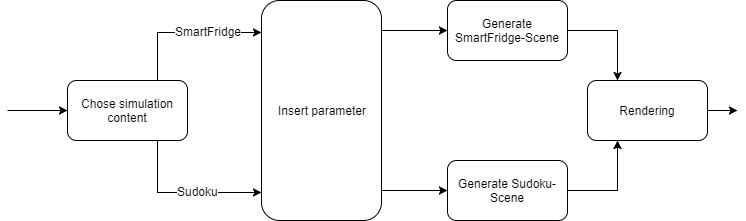
\includegraphics[scale=0.6]{sys_sw.png}
\end{figure}
\subsection{User Classes and Characteristics}
The following table contains the expected users and their characteristics.\\
\begin{tabular}{|l|l|l|l|}
\hline
\textbf{User} & Developer & Tester & External users \\
\hline
\textbf{Importance} & highest & high & low \\
\hline
\textbf{Usage extent} & Only specific feature & Only specific feature & All features \\
\hline
\textbf{Technical expertise} & high & high & low\\
\hline
\textbf{Frequency of use} & high & high & low \\
\hline
\textbf{Term of usage} & limited & short & long\\
\hline
\textbf{Description of usage} & The Developer will & Tester will use the & External users may\\
& use the simulation & simulation platform & use the software for \\ 
&  platform to design and  & form to test and & practical and/or.\\
&  validate their code. & validate specific & nonpractical use. \\
& & systems. & \\
\hline
\end{tabular}
\subsection{Operating Environment}
The generated images should primarily be readable and usable for the other project groups which use this to test their algorithms. Therefore, the software should run on common and available operating systems like Linux and/or Microsoft Windows. The results are stored in common file formats on these operating systems to grant the maximum possible compatibility.
\subsection{Design and Implementation Constraints}
\begin{itemize}
\item The software should run on any computerlike device and scale the scene according to the processor and RAM.
\item The required simulation time scales with the hardware of the operating system. It his highly recommended that a user is aware of his system's capabilities.
\item The software is exclusively available in an english version.
\item There will be no maintaining in excess of this lecture.

\end{itemize}
\subsection{User Documentation}
The following documents in pdf format will be available for users:
\begin{itemize}
\item User Manual.
\item Troubleshooting, FAQs.
\end{itemize}
\subsection{Assumption and Dependencies}
This particular software depends on the open sourced softwares Blender and FEniCS.
\newpage

\section{External Interface Requirements}
\subsection{User Interfaces}
The software provides a simple user interface as shown below:
\begin{figure}[H]
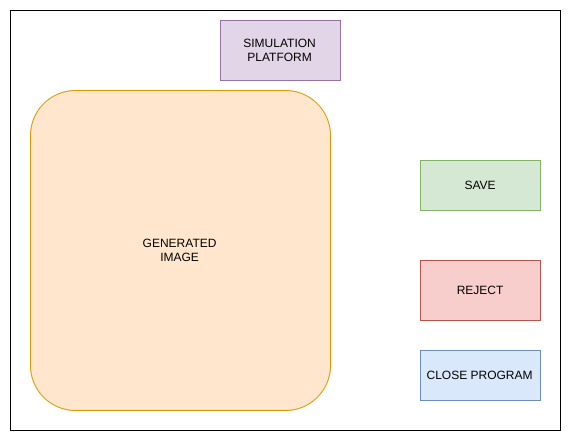
\includegraphics[scale=0.75]{gui.png}
\end{figure}
\subsection{Hardware Interfaces}
The systems works stand alone and the generated results are stored on the same hardware device.
\subsection{Software Interfaces}
The dataset generated from the hardware is passed on as an image data. 


\newpage
\section{System Features}
\subsection{Generate Images}
This feature pertains to generating a dataset of rendered images. It has highest priority.
\subsubsection{Stimulus/Response Sequences}
\begin{tabular}{|l|l|}
\hline
\textbf{Stimulus} & \textbf{Response} \\
\hline
User runs the software.	& Context dialogue shows up. \\
\hline
User selects content & parameter dialogue shows up. \\
\hline
User adjusts parameters. & Scene preview appears. \\
\hline
User confirms or rejects the generated scene. & \textbullet $\,$ Image is rendered and saved.\\
& \textbullet $\,$ New scene is generated. \\
\hline
\end{tabular}
\subsubsection{Functional Requirements}
\begin{itemize}
\item \textbf{REQ-1:} Simulate images based on the requirements from the projects: SmartFridge and Sudoku solver.
\item \textbf{REQ-2:} Display scene for user interaction.
\item \textbf{REQ-3:} Provide labels/annotations for selected images by the user.
\item \textbf{REQ-4:} Saving the selected images for future use.
\end{itemize}
\section{Other Nonfunctional Requirements}
\subsection{Performance Requirements}
\begin{itemize}
\item \textbf{REQ N-1.1:} Must run on a single core CPU with/without a GPU.
\end{itemize}

\subsection{Software Quality Attributes}
\begin{itemize}
\item \textbf{REQ N-2.1:} The software should be portable across systems and platforms.
\item \textbf{REQ N-2.2:} The software must be reliable enough such that there is not a huge disparity between the results generated from simulations and real images.
\end{itemize}

\section{Other Requirements}
In terms of license, we use GNU General Public License v2.0. The software can be used commercially, modified, distributed and can be used privately. We do not provide any liability or warranty for the software.
\end{document}
